 \documentclass[12pt,fleqn]{article}
\pagestyle{empty}
\usepackage[margin=2cm, top=3cm]{geometry} % Set margin and top spacing
\renewcommand{\thesection}{\Alph{section}} % Sections labeled as A, B, C...
\renewcommand{\thesubsection}{\arabic{subsection}} % Subsections labeled as 1, 2, 3...
\renewcommand{\thesubsubsection}{(\alph{subsubsection})} % Subsubsections labeled as (a), (b), ...
\usepackage{amsmath}
\usepackage{graphicx}
\usepackage{enumerate}
\setlength{\parindent}{0pt}
\usepackage{adjustbox}
\usepackage{tikz}
\usepackage{listings}

\usepackage{hyperref}
\usepackage{makecell}
\usepackage{caption}
\usepackage{subcaption}
\usepackage{float}
\usepackage{siunitx}
\numberwithin{subsection}{section}  


\begin{document}
\noindent 
\huge
\medskip
TU Berlin Robotics\\
\textbf{Lab Assignment \#4}\\

\normalsize
\noindent
\bigskip
Gruppe: 1\_Mon\_G \\
\medskip
\begin{tabular}[c]{|c|c|c|c|c|c|c|}
    \hline
    Student Name & B1 & C1 & C2 & C3 & C4 & C5\\
    \hline
    \hline
    Bryan Oppong-Boateng & X & X & X & X & X & X \\
    \hline
    Gökay Sengün & X & X & X & X & X & X \\
    \hline
    Jarne Jüchser & X & X & X & X & X & X \\
    \hline
    Caspar Siemssen & X & X & X & X & X & X \\
    \hline
\end{tabular}

\section{Bayes}
\subsection{}

\begin{align*}
P(open \mid z = 42) = \frac{P(z=42 \mid open) P(open)}{P(z = 42)}
\end{align*}

\begin{align*}
P(z=42) &= P(z=42 \mid open)P(open) + P(z=42 | \neg open) P(\neg open) \\
&= \frac{2}{3} \cdot \frac{3}{5} + \frac{1}{3} \cdot \frac{2}{5} \\
&= \frac{8}{15}
\end{align*}

\begin{align*}
P(open \mid z=42) &= \frac{\frac{2}{3} \cdot \frac{3}{5}}{\frac{8}{15}} \\
&= \frac{3}{4}
\end{align*}

\section{Mapping with Raw Odometry}
\stepcounter{subsection}
\subsection{}

\begin{figure}[H]
     \centering
     \begin{subfigure}{0.3\textwidth}
         \centering
         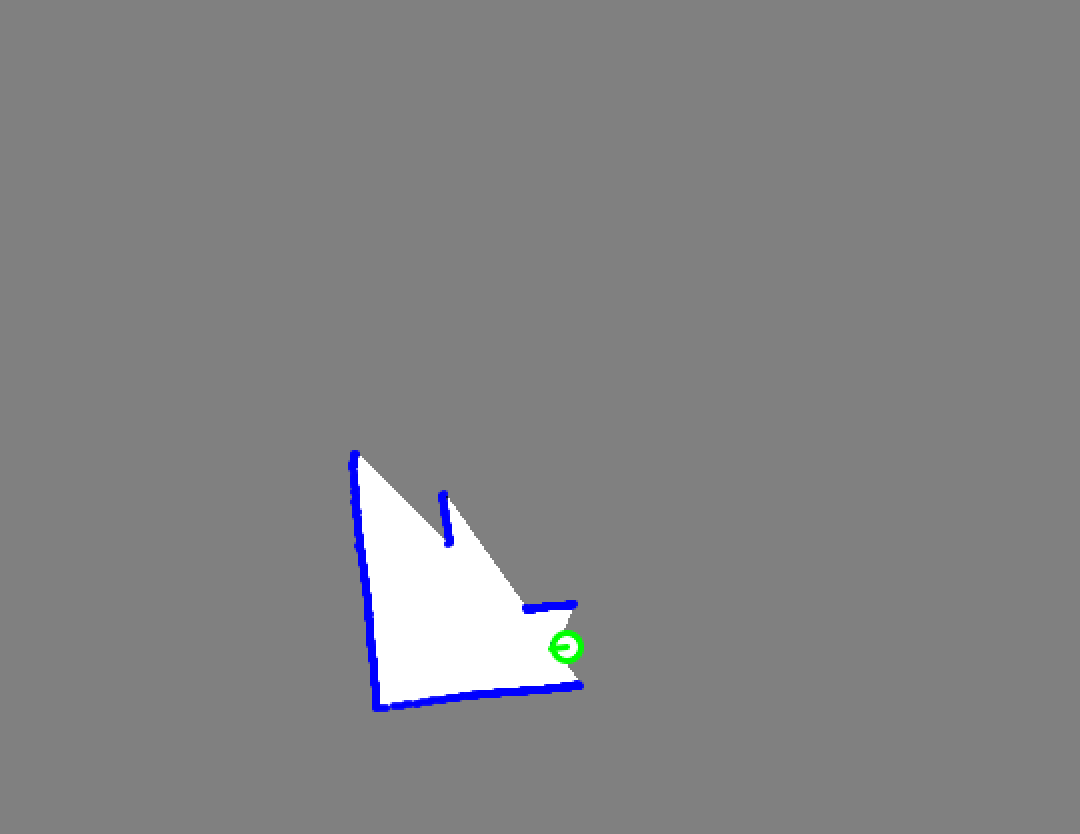
\includegraphics[width=\textwidth]{figures/mapping_2s.png}
         \caption{$t = \SI{2}{\second}$}
         \label{mapping2s}
     \end{subfigure}
     \hfill
     \begin{subfigure}{0.3\textwidth}
         \centering
         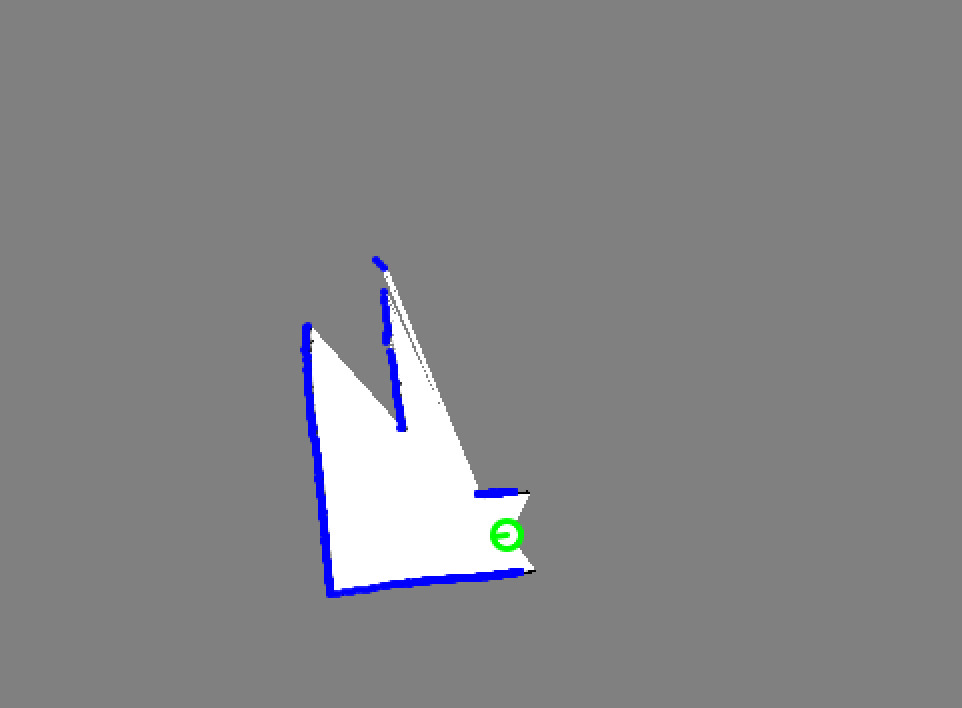
\includegraphics[width=\textwidth]{figures/mapping_8s.png}
         \caption{$t = \SI{8}{\second}$}
         \label{mapping8s}
     \end{subfigure}
     \hfill
     \begin{subfigure}{0.3\textwidth}
         \centering
         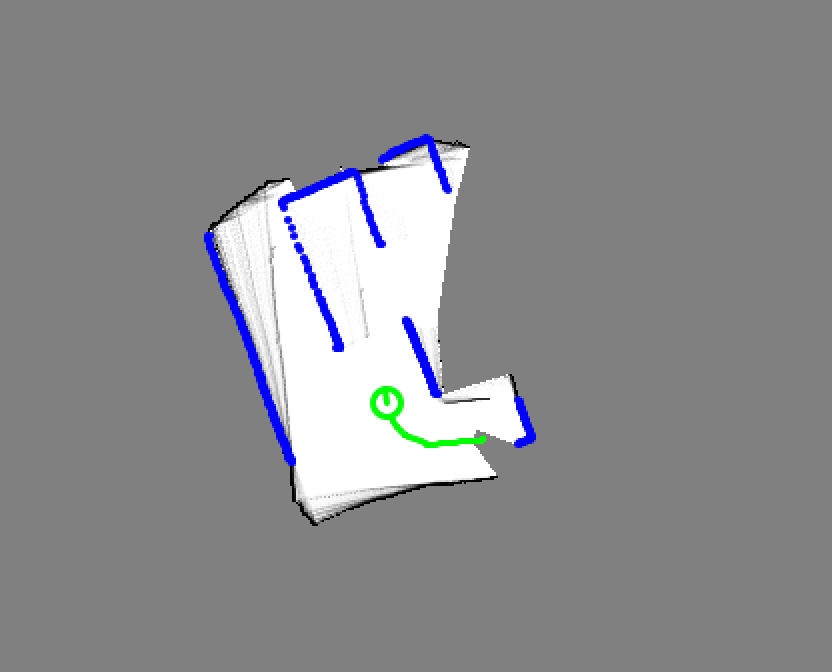
\includegraphics[width=\textwidth]{figures/mapping_20s.png}
         \caption{$t = \SI{20}{\second}$}
         \label{mapping20s}
     \end{subfigure}
        \caption{Mapping}
        \label{fig:three graphs}
\end{figure}

\subsection{}

The localization uses the current roboter pose in the map. Errors in the roboter pose are directly reflected in the map because the obstacles are drawn relative to the roboter pose. Therefore, it is important to have an accurate roboter pose which is not easy as there might be different error sources like slippage or inaccuracies in the robots movement. To improve this, one should do simultanious localization and mapping to increase the accuracy of the robot pose. 

\section{Monte Carlo Localization: Particle Filter}
\stepcounter{subsection}
\stepcounter{subsection}
\stepcounter{subsection}
\stepcounter{subsection}
\stepcounter{subsection}
\subsection{}
\subsubsection{}
\begin{figure}[H]
     \centering
     \begin{subfigure}{0.2\textwidth}
         \centering
         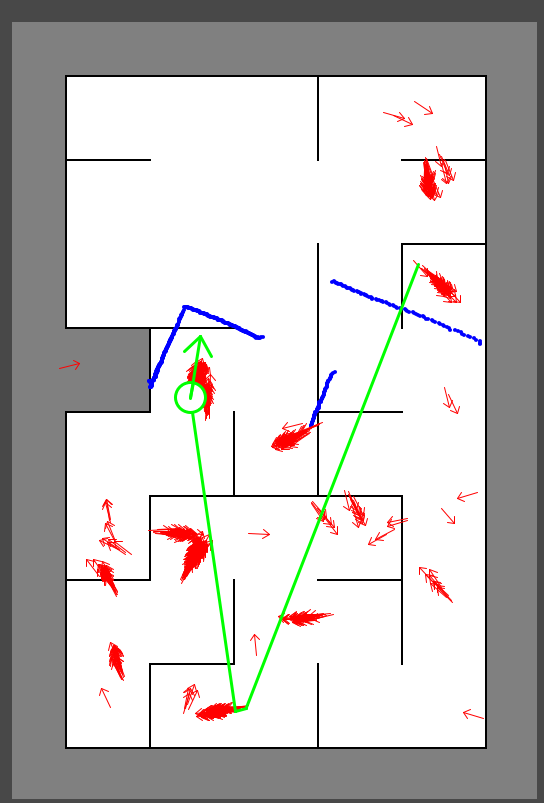
\includegraphics[width=\textwidth]{figures/localization_5s.png}
         \caption{$t = \SI{5}{\second}$}
         \label{mapping2s}
     \end{subfigure}
     \hspace{1em}
     \begin{subfigure}{0.2\textwidth}
         \centering
         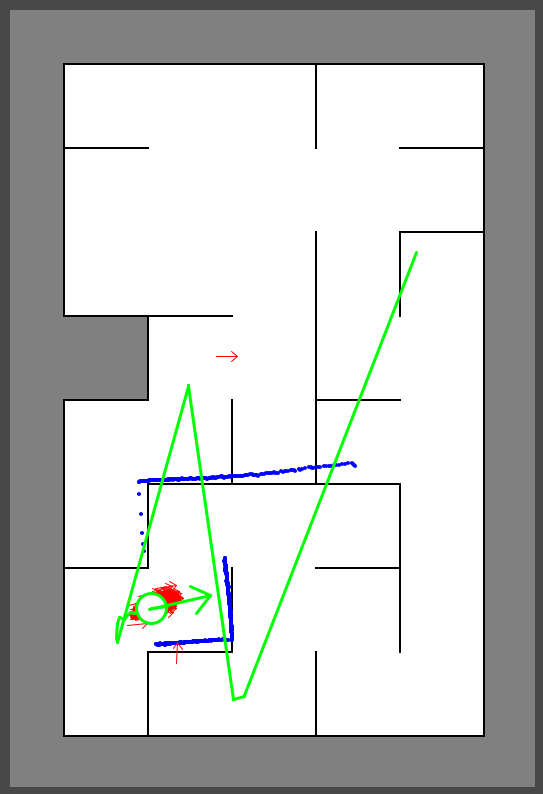
\includegraphics[width=\textwidth]{figures/localization_10s.png}
         \caption{$t = \SI{10}{\second}$}
         \label{mapping8s}
     \end{subfigure}
     \hspace{1em}
     \begin{subfigure}{0.2\textwidth}
         \centering
         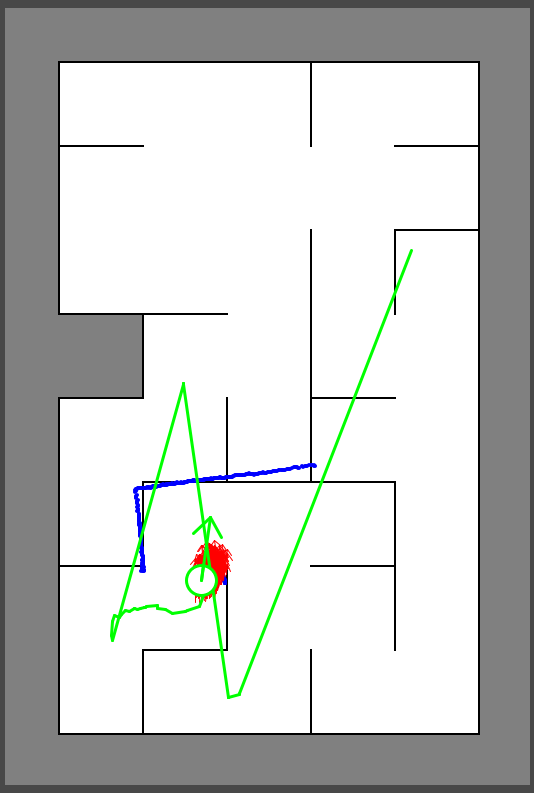
\includegraphics[width=\textwidth]{figures/localization_14s.png}
         \caption{$t = \SI{14}{\second}$}
         \label{mapping20s}
     \end{subfigure}\\
     \begin{subfigure}{0.2\textwidth}
         \centering
         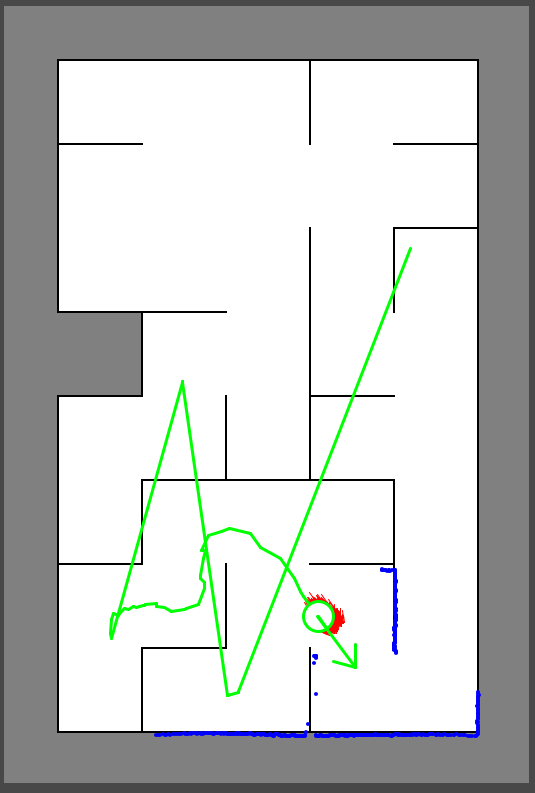
\includegraphics[width=\textwidth]{figures/localization_20s.png}
         \caption{$t = \SI{20}{\second}$}
         \label{mapping20s}
     \end{subfigure}
     \hspace{1em}
     \begin{subfigure}{0.2\textwidth}
         \centering
         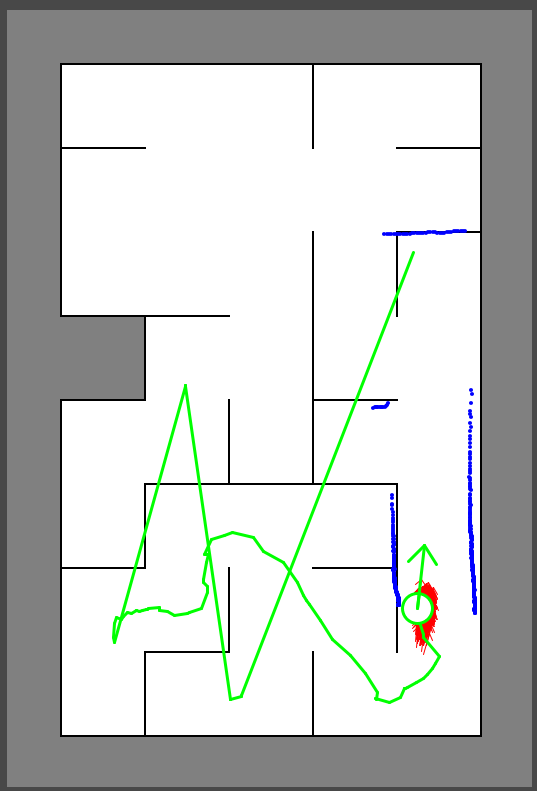
\includegraphics[width=\textwidth]{figures/localization_30s.png}
         \caption{$t = \SI{30}{\second}$}
         \label{mapping20s}
     \end{subfigure}
     \hspace{1em}
     \begin{subfigure}{0.2\textwidth}
         \centering
         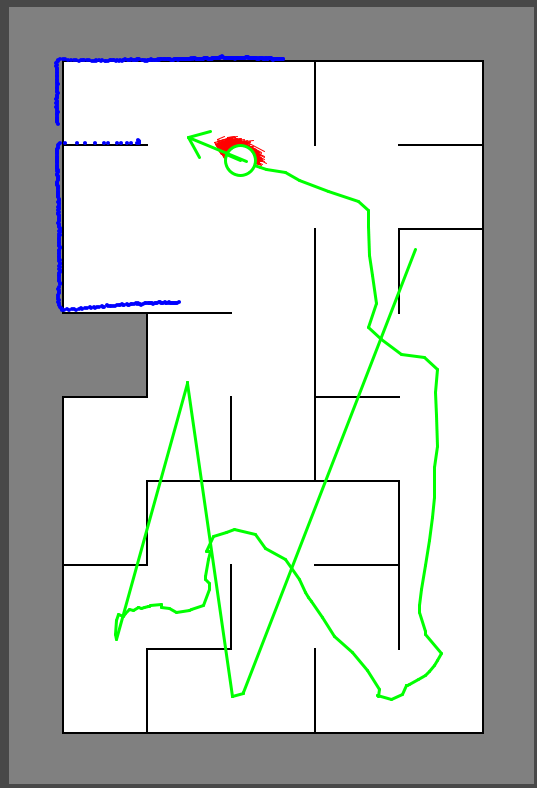
\includegraphics[width=\textwidth]{figures/localization_42s.png}
         \caption{$t = \SI{42}{\second}$}
         \label{mapping20s}
     \end{subfigure}\\
     \begin{subfigure}{0.2\textwidth}
         \centering
         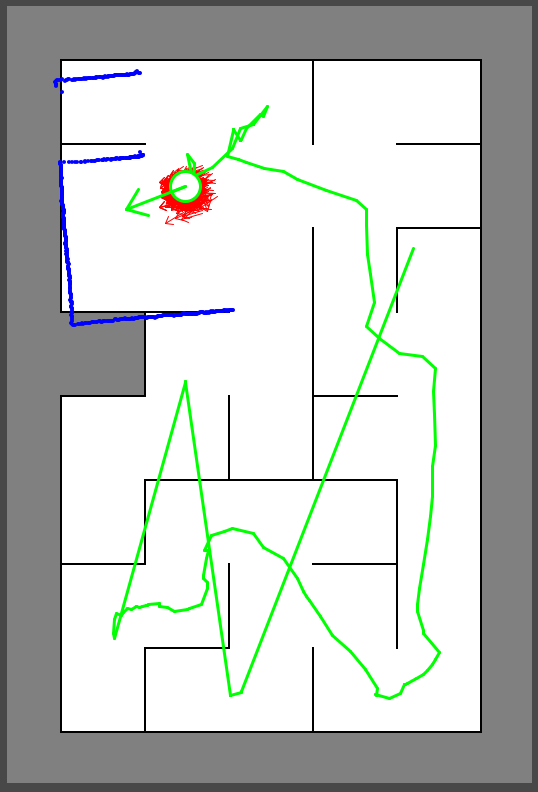
\includegraphics[width=\textwidth]{figures/localization_60s.png}
         \caption{$t = \SI{60}{\second}$}
         \label{mapping20s}
     \end{subfigure}
     \hspace{1em}
     \begin{subfigure}{0.2\textwidth}
         \centering
         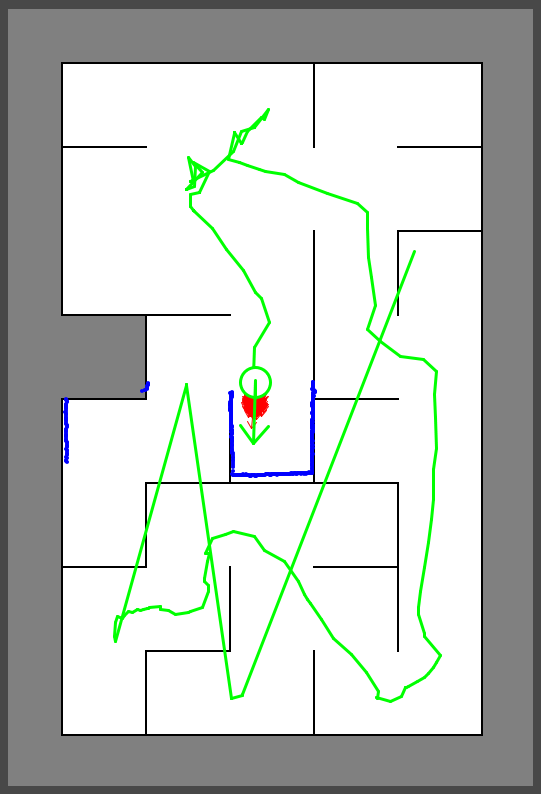
\includegraphics[width=\textwidth]{figures/localization_75s.png}
         \caption{$t = \SI{75}{\second}$}
         \label{mapping20s}
     \end{subfigure}
        \caption{Localization with uniform distribution}
        \label{fig:three graphs}
\end{figure}



\subsubsection{}
\begin{figure}[H]
     \centering
     \begin{subfigure}{0.2\textwidth}
         \centering
         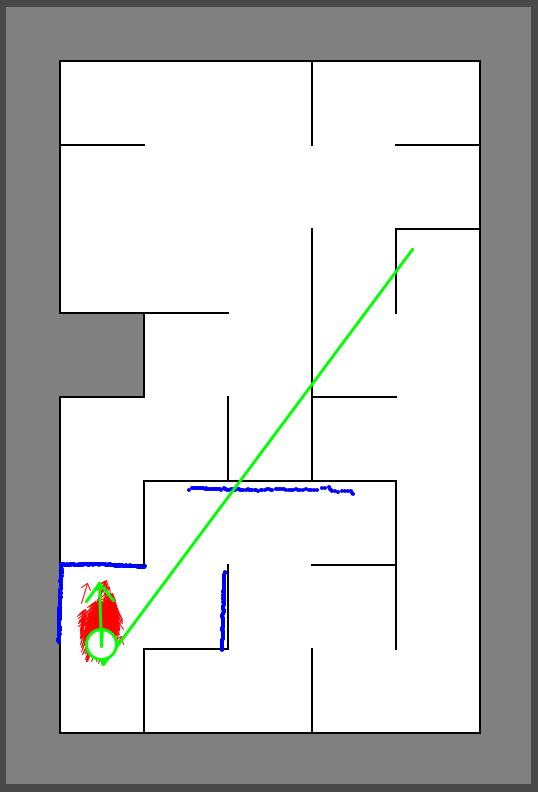
\includegraphics[width=\textwidth]{figures/localization2_5s.png}
         \caption{$t = \SI{5}{\second}$}
         \label{mapping2s}
     \end{subfigure}
     \hspace{1em}
     \begin{subfigure}{0.2\textwidth}
         \centering
         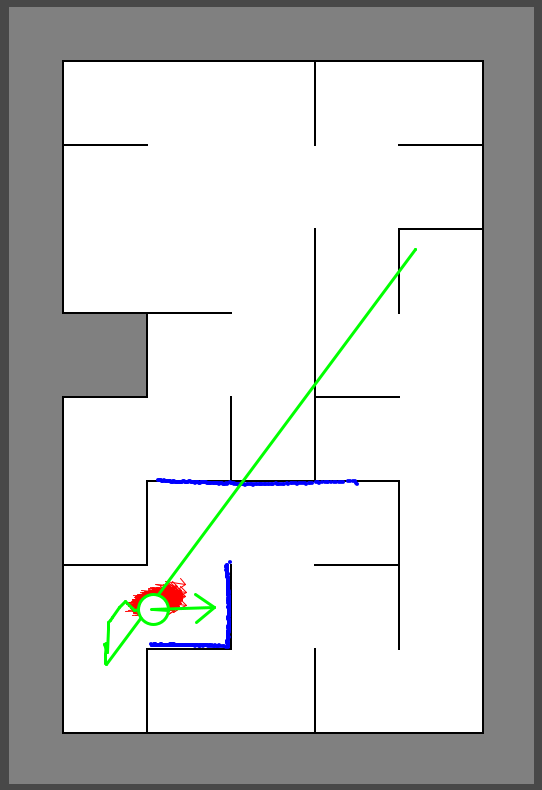
\includegraphics[width=\textwidth]{figures/localization2_10s.png}
         \caption{$t = \SI{10}{\second}$}
         \label{mapping8s}
     \end{subfigure}
     \hspace{1em}
     \begin{subfigure}{0.2\textwidth}
         \centering
         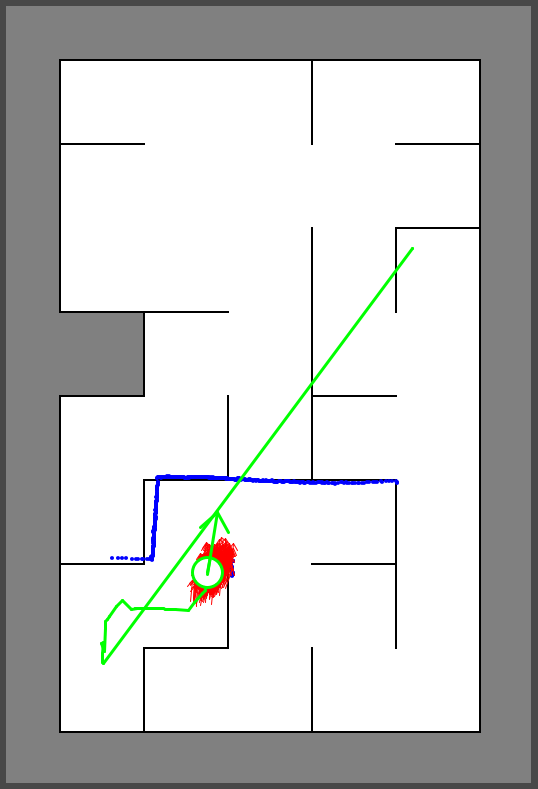
\includegraphics[width=\textwidth]{figures/localization2_14s.png}
         \caption{$t = \SI{14}{\second}$}
         \label{mapping20s}
     \end{subfigure}\\
     \begin{subfigure}{0.2\textwidth}
         \centering
         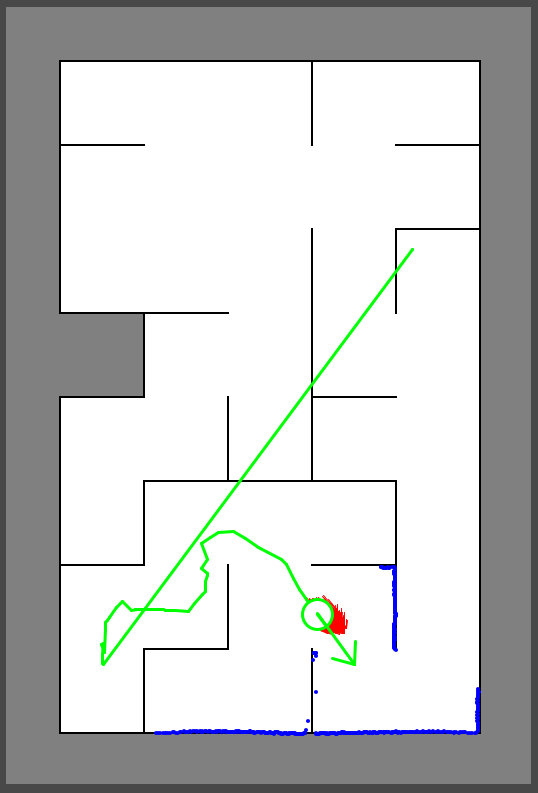
\includegraphics[width=\textwidth]{figures/localization2_20s.png}
         \caption{$t = \SI{20}{\second}$}
         \label{mapping20s}
     \end{subfigure}
     \hspace{1em}
     \begin{subfigure}{0.2\textwidth}
         \centering
         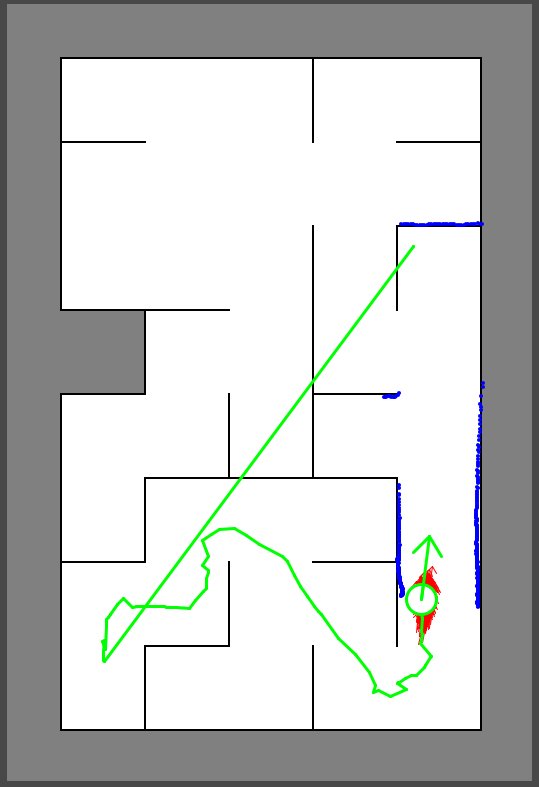
\includegraphics[width=\textwidth]{figures/localization2_30s.png}
         \caption{$t = \SI{30}{\second}$}
         \label{mapping20s}
     \end{subfigure}
     \hspace{1em}
     \begin{subfigure}{0.2\textwidth}
         \centering
         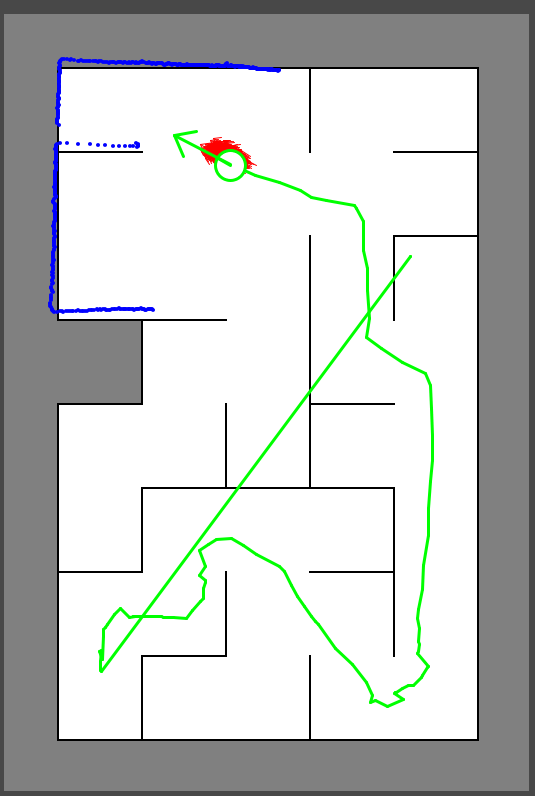
\includegraphics[width=\textwidth]{figures/localization2_42s.png}
         \caption{$t = \SI{42}{\second}$}
         \label{mapping20s}
     \end{subfigure}\\
     \begin{subfigure}{0.2\textwidth}
         \centering
         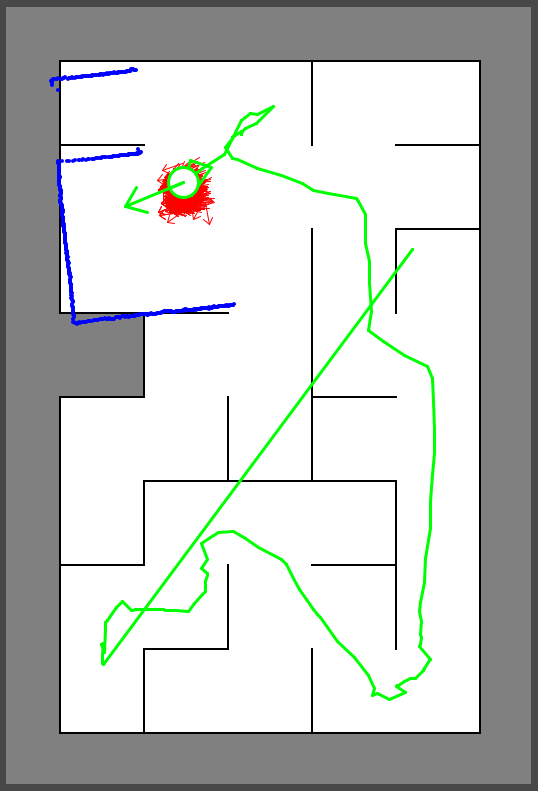
\includegraphics[width=\textwidth]{figures/localization2_60s.png}
         \caption{$t = \SI{60}{\second}$}
         \label{mapping20s}
     \end{subfigure}
     \hspace{1em}
     \begin{subfigure}{0.2\textwidth}
         \centering
         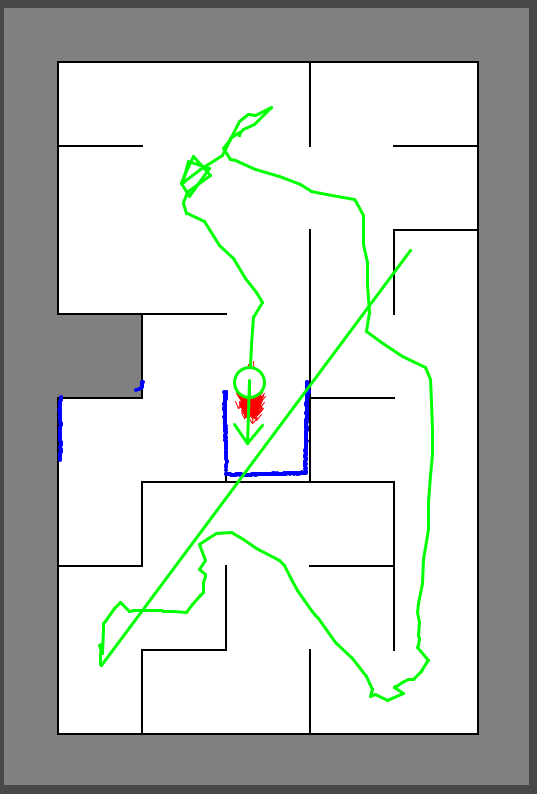
\includegraphics[width=\textwidth]{figures/localization2_75s.png}
         \caption{$t = \SI{75}{\second}$}
         \label{mapping20s}
     \end{subfigure}
        \caption{Localization with gaussian distribution}
        \label{fig:three graphs}
\end{figure}
\end{document}
